%%%%%%%%%%%%%%%%%%%%%%%%%%%%%%%%%%%%%%%%%
% Simple Sectioned Essay Template
% LaTeX Template
%
% This template has been downloaded from:
% http://www.latextemplates.com
%
% Note:
% The \lipsum[#] commands throughout this template generate dummy text
% to fill the template out. These commands should all be removed when 
% writing essay content.
%
%%%%%%%%%%%%%%%%%%%%%%%%%%%%%%%%%%%%%%%%%

%----------------------------------------------------------------------------------------
%	PACKAGES AND OTHER DOCUMENT CONFIGURATIONS
%----------------------------------------------------------------------------------------

\documentclass[12pt]{article} % Default font size is 12pt, it can be changed here

\usepackage{geometry} % Required to change the page size to A4
\geometry{a4paper} % Set the page size to be A4 as opposed to the default US Letter
\usepackage{listings} % Insert program segments in the text
\usepackage{float} % Allows putting an [H] in \begin{figure} to specify the exact location of the figure
\usepackage{wrapfig} % Allows in-line images such as the example fish picture
\usepackage[per-mode=fraction]{siunitx}
\usepackage{lipsum} % Used for inserting dummy 'Lorem ipsum' text into the template
\usepackage{graphicx}
\usepackage{multirow}
\usepackage[caption=false,font=footnotesize]{subfig}
\usepackage{dblfloatfix}
\usepackage{xspace}
\usepackage{url}
\usepackage{algorithm}
\usepackage{algorithmic}
\usepackage[algo2e]{algorithm2e}
\usepackage{amsmath}
\usepackage[table]{xcolor}
\usepackage{cite}
\usepackage{url}

\newcommand{\tabincell}[2]{\begin{tabular}{@{}#1@{}}#2\end{tabular}}

\linespread{1.2} % Line spacing
%\setlength\parindent{0pt} % Uncomment to remove all indentation from paragraphs

\graphicspath{{./figures/}} % Specifies the directory where pictures are stored

\begin{document}

%----------------------------------------------------------------------------------------
%	TITLE PAGE
%----------------------------------------------------------------------------------------

\begin{titlepage}

\newcommand{\HRule}{\rule{\linewidth}{0.5mm}} % Defines a new command for the horizontal lines, change thickness here

\center % Center everything on the page

\HRule \\[0.4cm]
{ \huge \bfseries BFS Accelerator}\\[0.4cm] % Title of your document
\HRule \\[1.5cm]

\begin{minipage}{0.4\textwidth}
    \centering {Cheng Liu} \\ 
    \vspace{2em}
    \centering {\large \today}
\end{minipage}

\end{titlepage}

%----------------------------------------------------------------------------------------
%	TABLE OF CONTENTS
%----------------------------------------------------------------------------------------

%\tableofcontents % Include a table of contents

%\newpage % Begins the essay on a new page instead of on the same page as the table of contents 

%----------------------------------------------------------------------------------------
%	INTRODUCTION
%----------------------------------------------------------------------------------------
\section{Motivation} % Major section
In the era of "big data", there has been growing interest in developing graph analytics 
applications to gain new insights and solutions. While Breadth-First Search (BFS) algorithm 
is the foundation for many graph processing applications and analytics workloads, many BFS 
acceleration designs have been proposed targeting multi-core processors, distributed systems, 
GPUs and FPGAs over the years as listed in Table \ref{table:bfs-literature}. 
FPGA which allows intensive application-specific customization 
has been well-known to be energy efficient compared to general purposed computing devices 
and is usually able to provide unique performance-energy trade-offs. However, the best 
performance of BFS accelerator reported in literature is only around \numrange{1}{2} billion 
traverses per second and is far behind that on the counterpart computing platforms 
which goes up to 120 billion traverse per second in spite of the memory bandwidth gap. 

\begin{table}[htb]
    \centering
    \caption{Brief BFS Acceleration Review\label{table:bfs-literature}}{
        \vspace{1em}
        \centering
        \resizebox{0.8\columnwidth}{!}{
            \begin{tabular}{l|l|l|l|l}
                \hline
                Name & Year & Platform & Memory Bandwidth & Performance \\ \hline
                Enterprise \cite{liu2015enterprise} & 2015 & GPU & \tabincell{l}{300GB/s \\ 600GB/s}  & \tabincell{l}{76 GTEPS \\ 122 GTEPS} \\ \hline
                ASAP12 \cite{betkaoui2012reconfigurable} & 2012 & FPGA  & 80GB/s & 1.6 GTEPS  \\ \hline
                IPDPSW14 \cite{attia2014cygraph} & 2014 & FPGA & 80GB/s & 1.9 GTEPS \\ \hline 
                FPL15 \cite{umuroglu2015hybrid} & 2015 & FPGA & 3.2GB/s & 0.172 GTEPS \\ \hline
                GraphOps \cite{oguntebi2016graphops} & 2016 & FPGA & 38GB/s & 0.8 GTEPS ? \\ \hline 
                Graphicionado \cite{ham2016graphicionado} & 2016 & ASIC & 68GB/s & --? \\ \hline
                GraVF \cite{engelhardt2016gravf} & 2016 & FPGA & -- ? & 3.8GTEPS \\ \hline
            \end{tabular}
        }
    }
\end{table}

When comparing the BFS accelerators on FPGA and GPU, we observe that existing FPGA accelerators 
mainly fall short on two aspects. First of all, the BFS accelerators on FPGAs have lower 
memory utilization which is critical to the resulting BFS performance because BFS is a 
memory-bound computing task due to the irregular memory access. Although the memory utilization 
may be influenced by many different factors such as the memory hierarchy and processing power 
difference, one of the primary factors is the amount of memory access needed for the same BFS task. 
The BFS accelerators on FPGA have few efficient BFS algorithmic strategies supported 
which are considered to be effective for alleviating the memory bandwidth bottleneck. For example, 
the adaptive top-down and bottom-up BFS strategy infers the BFS frontier from the 
visited vertices at the beginning of BFS while doing so from the unvisited vertices 
when the BFS frontier gets large. Basically, this strategy helps to reduce the amount 
of memory access while detecting the BFS frontier. Another example is the 
high degree vertex caching. Vertices with high degree will be cached locally, which can be used 
to avoid accessing main memory during the traverse and thus also helps alleviate memory 
bandwidth pressure. With appropriately applying the algorithmic BFS strategies, the memory 
utilization of the BFS accelerators can be enhanced and thus the performance can be improved 
eventually.

Secondly, the practical graphs are typically scale-free and the vertex degree 
varies in a large range. As a result, the exploration of different type of vertices 
may require diverse exploration time. When they are assigned to the processing engines of BFS, 
the parallel processing engines allocated with low-degree vertices may be under utilized. 
In addition, inspecting low-degree vertices requires scattered short read over the 
CSR data stored in main memory while inspecting high-degree vertices mostly has continuous 
burst memory access. To approach this problem, unlike previous work which usually 
have homogeneous processing engines implemented on FPGA, we may classify the vertices in 
the frontier based on the degree of the vertices and allocate them to specifically customized 
processing engines accordingly. Meanwhile, with appropriate resource allocation, we may 
statically (or dynamically) adjusting the number of processing engines for different 
vertices such that the utilization of the processing engines can be balanced.

\section{Proposed BFS Accelerator}
In this section, the proposed BFS accelerator will be illustrated. It 
follows the classical BSP model. Basically it will traverse the vertices 
iteratively from the starting vertex. It will not proceed to the next iteration 
before all the active vertices (frontier) are explored in current iteration.

\subsection{Background}
Before illustrating the proposed BFS accelerator, we will explain the basic concept 
of BFS with a basic BFS implementation shown in List \ref{lst:seq-bfs}. Suppose $depth[v]$ represents the 
depth of vertex $v$ in a graph $G$. $s$ stands for the starting vertex of the Graph $G$. 
Then the sequential BFS algorithm is described as follows. 

\begin{lstlisting}[caption={Sequential BFS Algorithm}, label={lst:seq-bfs}, language=c, showstringspaces=false]
// top-down BFS algorithm
depth[s] = 0;
level = 0;
// Overall iteration control
while(!bfsIsDone(level)){
    // Inspect depth data and find the vertices in the frontier
    for(v in G){
        if (depth[v] == level){ 
            // Expand the vertices in the frontier
            for (v' in v.successor()){
                // update v' depth  if it is unvisited
                if(depth[v'] == inf){ 
                    depth[v'] = level + 1;
                }
            }
        }
    }

    // Proceed to the next iteration
    level++;
}

// When the frontier is empty, the bfs completes.
bool bfsIsDone(level){
    int counter = 0;
    for(v in G){
        if (depth[v] == level)
            counter++;
    }
    if(counter == 0) return true;
    else return false;
}

\end{lstlisting}

Given the algorithm presented above, the BFS can be roughly divided into 
the following three phases:

\begin{itemize}
    \item Phase 1: Get the frontier queue based on the status array 
        (or the depth of the graph) and completes the BFS when the queue is empty. 
    \item Phase 2: Traverse the successors of vertices in the frontier. 
    \item Phase 3: If the successors are unvisited, update its depth information 
        and mark it as visited. When all the vertices in the frontier are explored, 
        move to the next iteration.
\end{itemize}

\subsection{Proposed Parallel BFS}
With the sequential BFS, we can further parallelize it. As shown in \ref{lst:parallel-bfs},  
we keep the same three-phase design and have each phase parallelized and optimized. 
The details can be found in the comments in the algorithm. On top of the optimizations presented 
in the algorithm, we still need to perform the adaptive top-down and bottom-up switching.
It requires minor modifications on most of the basic processing in the algorithm and is omitted for 
simplicity. 

\begin{lstlisting}[caption={Parallel BFS Algorithm}, label={lst:parallel-bfs}, language=c, showstringspaces=false]
depth[s] = 0;
level = 0;
// Overall iteration control
while(!bfsIsDone(level)){
    // Phase 1: Inspect depth of all the vertices 
    // for frontier vertices, classify the 
    // frontier vertices into three types, and 
    // have them stored in three different 
    // queues respectively. Meanwhile, visited hub 
    // vertices (vertices with high degree) will be 
    // cached on chip and it will be used in the 
    // following processing. In addition, 
    // the inspecting process can be divided into multiple 
    // independent tasks as well.
    for(v in G){ 
        if (depth[v] == level){
            if(v.outDegree() < 32){
                smlQueue.push(v);
            }
            else if(v.outDegree() < 256){
                midQueue.push(v);
            }
            else{
                lrgQueue.push(v);
            }
        }
        // Store visited hub vertices into on chip cache.
        else if(depth[v] < level and v.degree() > 1024){
            HubVertexCache(v);
        }
    }

    // Phase 2: Expand the vertices in the 
    // frontier. If the successors of 
    // the vertices haven't been visited yet, 
    // they will be send to a update queue 
    // corresponding to its depth location. 
    // Basically the vertices in 
    // different queues can update their depth 
    // in parallel. Vertices in the same queue 
    // may probably be reordered for potential 
    // consecutive write operation. 
    // Meanwhile, the expansion on each frontier 
    // queue can also be partitioned for parallel 
    // processing.
    for (v in smlQueue){
        for (v' in v.successor()){
            // If v' is found in HubVertexCache, 
            // it means it is visited and thus there is no 
            // need reading depth[v'] from memory for 
            // checking if it is visited.
            if(HubVertexCache[v'] hit){ 
               continue; 
            }
            // update v' depth  if it is unvisited
            else if(depth[v'] == inf){
                updateQueue[mod(v', backNum)].push(v');
            }
        }
    }

    // Phase 3: Update depth of the vertices 
    // in each updateQueue. As there may redundant 
    // vertices in each updateQueue which may eventually 
    // results in repeated memory write wasting 
    // memory bandwidth. Thus we need to 
    // remove the redundant vertices before 
    // writing back, though there is no guarantee 
    // squeezing all the redundant vertices.
    removeRedundantVertices(updateQueue);
    for (v in updateQueue){
        v.depth = level + 1;
    }

    // Proceed to the next iteration
    level++;
}
\end{lstlisting}

Here is summary of the optimization strategies of the proposed BFS algorithm 
targeting BFS accelerator design on FPGA or ASIC.
\begin{itemize}
    \item Frontier queue inspection partition for parallel processing.
    \item Frontier vertices classification based on vertex degree.
    \item Hub vertices caching to avoid repeated memory access.
    \item Application specific processing logic for different types of 
        vertices (i.e. vertices in different queues)
    \item Frontier queue partition for both parallel expansion and balanced expansion time.
    \item Reordering vertices to be updated to assist the parallel and consecutive depth update.
    \item Removing redundant vertices in each update queue compromising the hardware 
        overhead and saving memory bandwidth.
\end{itemize}

\subsection{The Proposed BFS Accelerator}
Here is the overview of the proposed BFS accelerator \ref{fig:bfs-overview}. The three phases of the 
BFS is implemented as three different pipeline stages. Basically, the figure 
visualizes parallel BFS algorithm. We will not repeat the details that have been explained 
in previous subsection. Here we will introduce the data storage in the accelerator. 
All the input data including 
CSR data and depth information will be stored on DDR directly. While the queues are needed 
to connect the pipeline stages and handle the mismatched processing speed at run-time.
In this figure, we assume that the frontier queue between the first pipeline and the second 
pipeline is implemented on DDR while the queues between the second and the third pipeline 
utilizes the on-chip storage.

Using DDR as the queue allows the relevant pipeline stages to operate on a 
larger data set but consumes larger memory bandwidth. Using the on-chip storage 
for buffering the intermediate data may miss some of the optimized design options, 
but it will save the on-chip memory bandwidth in general. Here we just show both the possible 
design options. Probably, the second option may be better, but anyway we will see 
the experiments in future.  

As the top-down method needs to traverse the successors of the frontier vertices while the 
bottom-up method needs to traverse the predecessors of the frontier, we need to store both of them 
in CSR for the adaptive method. 

\begin{figure}[tb]
\centering
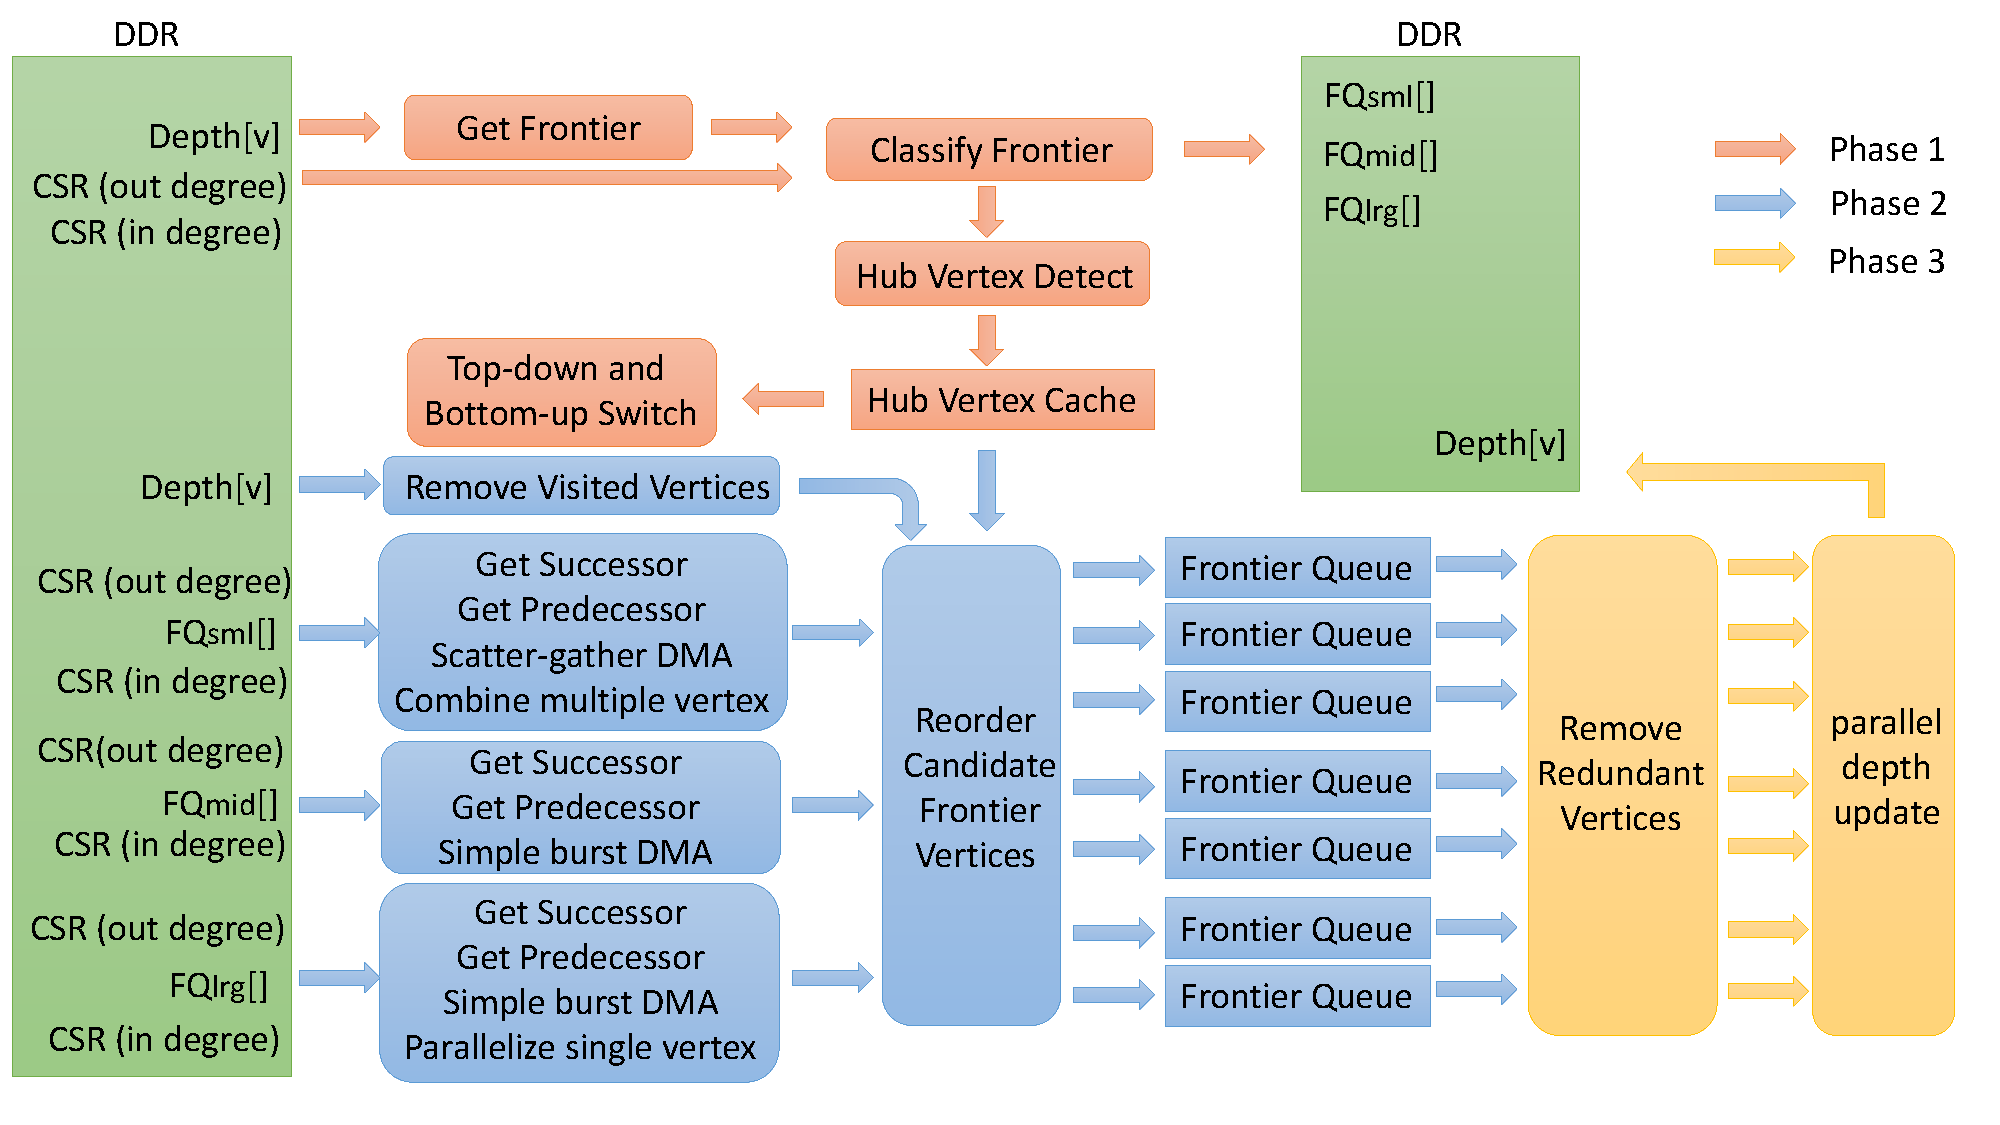
\includegraphics[width=0.9\linewidth]{bfs-overview}
\caption{BFS Overview, it consists of three pipelined phases. As the design follows the BSP model, 
    it will not move to the next iteration until Phase 3 completes. }
\label{fig:bfs-overview}
\vspace{-1em}
\end{figure}


\section{About the Experiments}
I am trying to develop a cycle-accurate simulator using SystemC first so that the design 
optimization techniques can be easily verified and evaluated. When the optimization techniques 
are decided, I can further build the real hardware design on the FPGAs with the most effective 
optimization techniques. I am not sure if it is a good idea to integrate all the optimization 
techniques in a single FPGA design. Maybe we can focus on one or two of them at a time for example the 
hub vertex caching and gradually extend the work. 

On top of the BFS accelerator optimization, another 
thing that I want to explore is how the BFS accelerator scales with the memory bandwidth. As the 
BFS accelerator is sensitive to the memory bandwidth and different FPGA platforms may have various 
memory bandwidth available, it may be interesting to develop a bandwidth-aware BFS accelerator or 
an auto-tuning framework over the existing BFS accelerator design for different FPGA platforms.  

As there is no available SystemC DRAM model, I planned to use DRAMSim2 as the model first. Then I found a 
new simulator ramulator developed by Prof. Mutlu's group \cite{kim2016ramulator}. It supports many different memory architectures 
including DDR series, LPDDR series, HBM etc. So I decided to use it instead. Hopefully, we may further extend this work to general graph accelerator design with new memory systems such as 3D-DRAM etc.   

%----------------------------------------------------------------------------------------
%	BIBLIOGRAPHY
%----------------------------------------------------------------------------------------
\bibliographystyle{plain}
\bibliography{refs}
%----------------------------------------------------------------------------------------

\end{document}
